\chapter{Frequecy Response Analysis}

So far the literature discussed in this book is conserned with the time response analysis using a step input. The time response analysis of dynamical system is limited to simple inputs such as step input or impulse input and so is the control design techniques used in pole placement and root locus methods. In general, there are complex signals given to a dynamical system and therefore a sperate analysis of such complex signal has to be studied separtely. In frequency response, analysis of system behavior is studied using complex repetitive signals such as sinusiodal waves. For a quick understanding of frequency response of a dynamical system, the analytical solution can be consdiered where there is both a transient respone (due to natural system dynamics) and a particular response (due to forcing functions) as shown in figure \ref{Fig_FreqResp_GrapSol}.
\begin{figure}[h!]
	\centering
	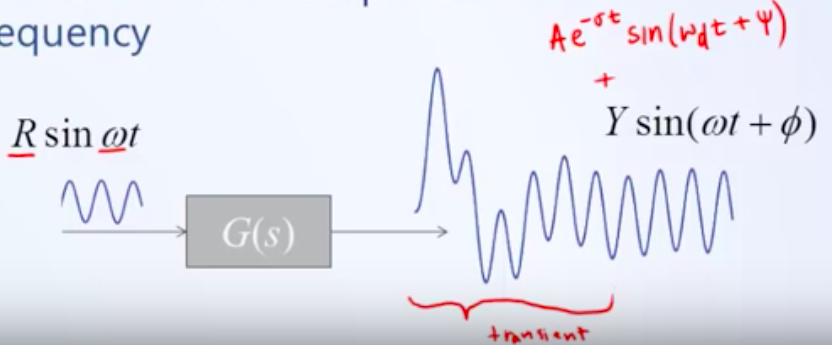
\includegraphics[width=0.5\linewidth]{Bilder/FrequencyResponse_GraphicalSolution}
	\caption{Graphical Represenataion of the Analytical frequency response}
	\label{Fig_FreqResp_GrapSol}
\end{figure}
Where the terms in black are the input and the ss system resposne (particluar solution) of the system. The term in red is the null solution (transient) of the system. As the null solution is a fucntion of $e^{-\sigma}$, where $\sigma$ is a real part of the complex number. It can be seen that this null part goes to zero leaving behaid only the particualar solution (ss response).
For a linear and a stable system (given input of a sinusiodal freqency), after the transients have been died out, the systems steady-state response will also be a sinusiodal output (particular solution) but might have a different magnitude (scaling with input) and could also have a phase shift with the input signal. In frequency response analysis, a study is conducted in order to determine such maganitude and phase anlge differences between the input signal and the response of the system.

In frequency rewsponse there are only two primary quanlities that have implications on the system performace:
\begin{enumerate}
	\item Scaling: The scaling of the magnitude of the system response to the input signal.
	\item Phase shift: The delay in the response of the systems response to the input signal.
\end{enumerate}

Generally, these two parameters are detemrined using experimental data, they can also be calculated using the TF $G(s) = G(j\omega)$. where $s = j \omega$, considering the frequencies of the system only. Therefore, the magnitude is determined by $|G(j \omega)|$ (ie., caclulating the magnitude of a complex number (generally pythogorean theorem)) in which case you should get $\omega$ of the systems frequency. Similarly, the phase shift can be determined by caculating the angle of the complex number $\angle G(j\omega)$ from the Re axis (generally calculated using atan).

Frequency analysis can help decide system behavior on various aspects: \label{List_FreqResp_Behavior}
\begin{enumerate}
	\item Attenuation: It could be both desired or undesired for the signal from the control system to be attenuated.
	\begin{itemize}
		\item Desired: In cases of noise cacellation and disturbace rejections (in some cases attenuation of control signal towars external disturbances is desired).
		\item Undesired: In cases where the control signals does not track the commanded reference signal.
	\end{itemize}
	\item Amplification: Can destabilise the system (may cause resonance)
	\item Phase lag: Information can be delayed which would cause the decay in the performace or could also destabilize the system.
\end{enumerate}

One of the ways to present this information is done using several different diagrams:
\begin{enumerate}
	\item Bode Diagram (two graphs)
	\begin{itemize}
		\item magnitude vs. frequency
		\item phase vs. frequency
	\end{itemize}
	\item  Nyquist plot (single plot)
	\begin{itemize}
		\item  manitude vs. phase (polar)
	\end{itemize}
	\item  Nicholas chart (single plot)
	\begin{itemize}
		\item  manitude vs. phase (rectangular)
	\end{itemize}
\end{enumerate}

\section{Plotting bode plots}

Bode plots basicaly describe the frequeny response of a dynamical system (magnitude and phase shifts) with reference to an input signal. As described in the previous section, these magnitude and phase shift of linear and stable system determine their various behavior and therefore, the response of the system as described in the lists \ref{List_FreqResp_Behavior}. In order to determine any of these system responses with reference to an input frequency, the magnitude and phase shift of the system response can be determined using Bode plots. There are two ways of plotting Bode plots, point by point (Matlab approach) and Line approximation approach (quick drwaing method on paper).

\subsection{Approach 1: Point-by-Point approach}

With point by point approach, Matlab calculates the individual magnitude and phase shifts at every input frequency through a brute force method using maganitude and angle calculations of the complex numbers. In the brute force method, substitute $s = j\omega$ into $G(s)$ and calculate magnitude and phase for series of different input frequencies $\omega$. The magnitude is sclaed to a log-log scale so as to incorpate the whole range of frequencies and multiplied by a factor of 20 (not sure why?) as follows:
\begin{equation}
	M (\omega) in dB = 20 log_{10}|G(j \omega)|
\end{equation}
Consider a PT-1 system,
\begin{equation}
	G(s) = \frac{1}{\tau s + 1}
\end{equation}
In order to determine the magnitude of this systems response, substitute $s = j \omega$ at every $\omega$ and perform the complex number caculation.
\begin{equation}
	G(j\omega) = \frac{1}{\tau j \omega + 1}
\end{equation}
taking the log scale and multiplying by a factor of 20, the above equation takes the form:
\begin{align*}
	20 log_{10} (G(j \omega)) &= 20 log_{10} \left( \frac{1}{\tau j \omega + 1} \right) \\
								&= 	20 log_{10} (1) - 20 log_{10} (j \omega + 1) \\
								&= 0 - 20 log_{10} (j \omega) - 20 log_{10} (1) \\
								&= - 20 log_{10} (j \omega)
\end{align*}
Phase shift can be determined calculating angle of the complex numbers:
\begin{equation}
	\phi (\omega) in deg = \angle G(j \omega)
\end{equation}

Alternatively, the magnitude and phase angle can be also determined using geometry:
\begin{equation} \label{Eq_FeResMagEquation}
	|G(j \omega)| = \sqrt{Re(G(j \omega))^{2} + Im(G(j \omega))^{2}}
\end{equation}
\begin{equation} \label{Eq_FeResPhaseEquation}
	\angle G(j \omega) = tan^{-1}\left( \frac{Im(G(j \omega))}{Re(G(j \omega))} \right)
\end{equation}

\subsection{Straight line approximations}

This approach is a rough sketch of the frequecy response hand drawn in order to derive a quick apprximation of the response. This is derived using standard results for each of the terms such as constants, poles or zeros at origin or at other places and summing up their results. This method is good for understanding quickly the systems response before hand and improves anlytical understanding.

It is important to know the most important standard results of various Bode plots from different components such as integrator, differentiator, gain, poles and zero in order to draw conclusions from the given Bode plot about the system. Studying system responses from different components helps to understand the system components responsible for such Bode plot generation during system identification.

In this straight line approximation technique, the response of individual componets is first determined on the Bode plot and then each of the individual responses is added together using some mathematical properties. For example consider a system given by its TF:
\begin{equation}
	G(s) = \frac{10 s}{s + 10}
\end{equation}
this system can be decomposed into its individual components such as:
\begin{equation}
	G(s) = (10) (s) \left( \frac{1}{s + 10} \right)
\end{equation}
where $10$ is the gain, $s$ is the differentiator and $1 / (s + 10)$ is the pole of the system. Since the magnitude response in plotted on the logarithemic scale as $dB$ on Bode plots, the summation porperty of the magnitude responses can be described as follows:
\begin{align}
	magnitude &= |G_{1}(j\omega) G_{2}(j\omega)| = |G_{1}(j\omega)||G_{2}(j\omega)| \\
	\implies log(|G_{1}(j\omega)||G_{2}(j\omega)|) &= log(|G_{1}(j\omega)|) + log(|G_{2}(j\omega)|) \label{Eq_FreqResp_LogAddProp}
\end{align}
From equation \eqref{Eq_FreqResp_LogAddProp}, it can be seen that on the logarithemic scale, the response of each component can be added linearly for the entire system as given by equation \eqref{Eq_FreqResp_LogAddProp}.

In case of phase response, the phase is not plotted on the logarithemic scale, rather the mathematical properties of complex numbers is used as described below:
\begin{equation}
	phase = \angle G_{1}(j \omega) G_{2}(j \omega) = \angle G_{1}(j \omega) + \angle G_{2}(j \omega) \label{Eq_FreqResp_ComplexNumsProp}
\end{equation}
The above equation \eqref{Eq_FreqResp_ComplexNumsProp} holds good as two complex numbers when multiply each other the result is given by their linear sum. Therefore, this mathematical proofs are used in order to construct a Bode plot for straight line approximations.

\subsubsection{Bode plot of Gain $K$} \label{Sec_BodePlotGain}

When the component is a simple gain $K$, then the magnitude will only be scaled up by the value of $K$. The phase will depend on the sign of $K$. If $K$ is positive, then phase = $0^{\circ}$ or when $K$ is negative, then the phase will be $180^{\circ}$ as shwon in figure \ref{Fig_FreqResp_BodePlot_K}. The magnitude will remian same weather $K$ is positive or negative, only the phase would change.
\begin{figure}[h!]
	\centering
	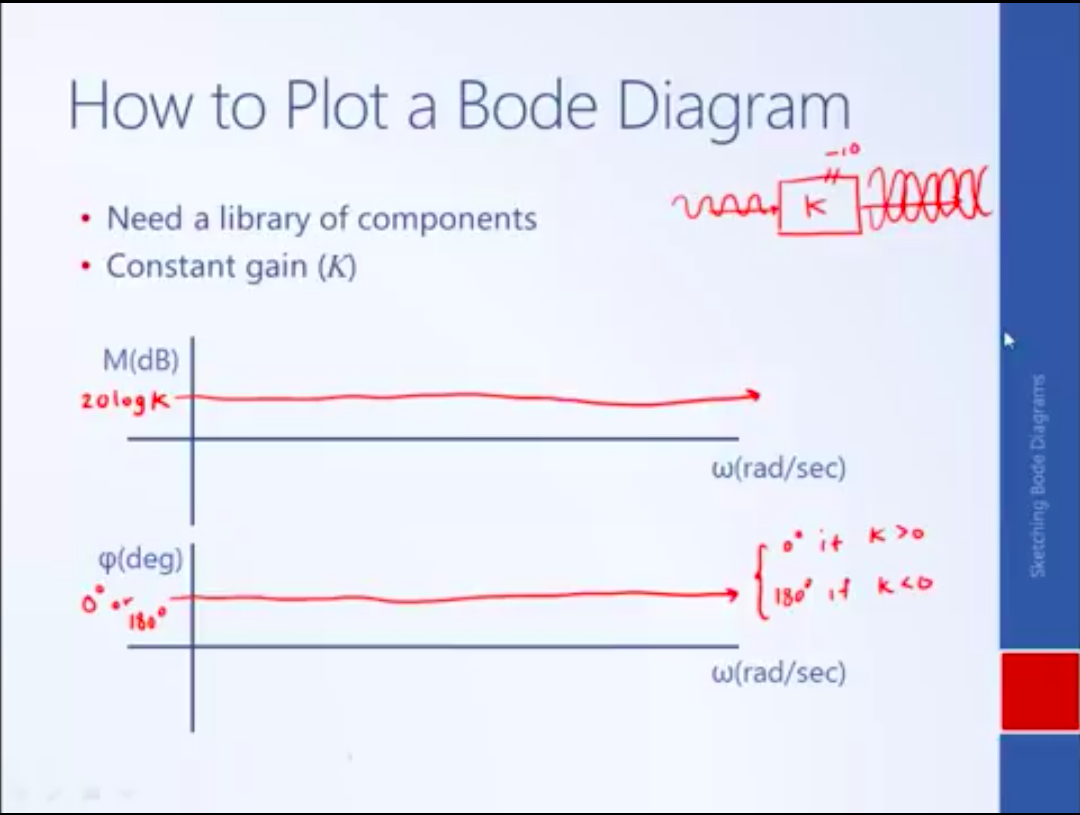
\includegraphics[width=\linewidth]{Bilder/FreqResp_BodePlot_K}
	\caption{Bode plot of gain $K$}
	\label{Fig_FreqResp_BodePlot_K}
\end{figure}

\subsubsection{Bode plot of Differentiator $s$}

The magnitude response of the Differentiator can be determined by substituting values of $s = j \omega$ in the TF $G(s)$. For a case when the number is purely imaginary, $s = j \omega$, as the value of $\omega$ increases, the value on the Im axis also increases ($j$ is to only denote that the value is on the Im axis). Because the magnitude of $j \omega$ is increasing there should be a slop to this line, in straight line approximation this slope is considered constant and therefore, the magnitude increases linearly. Further, at $ \omega = 1$ rad/s, $|G(j \omega)| = 20 log(1) = 0 dB$ at every multiple of $\omega$ to $10$ rad/s (a decade), the magnitude will be $|G(j \omega) = 20 log(10)| = 20 dB$. Therefore, the slope will be a constant (linear) of $20 dB/decade$ as shown in figure \ref{Fig_FreqResp_BodePlot_s}. Similarly, for every factor of $\omega$ in 10 rad/s, the slope will be continue backward with a slope value of $20 dB/decade$, therefore, the magnitude at $0.1$ rad/s will be $-20 dB$ as shown in figure \ref{Fig_FreqResp_BodePlot_s}.
\begin{figure}[h!]
	\centering
	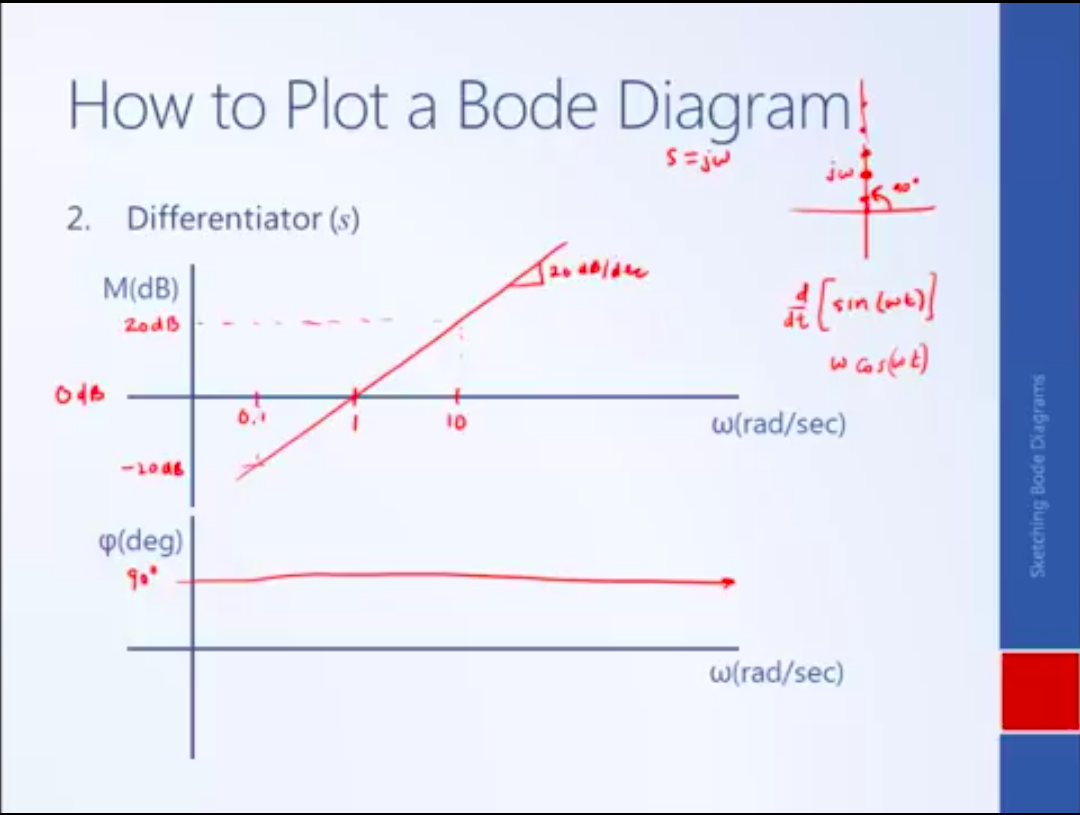
\includegraphics[width=\linewidth]{Bilder/FreqResp_BodePlot_s}
	\caption{Bode plot of Differentiator $s$}
	\label{Fig_FreqResp_BodePlot_s}
\end{figure}
Further, the phase of the differentiator will always be $90^{\circ}$ as $s = j \omega$ will always be on the positive of Im axis (negative $\omega$ does not exit physically, there could be a sign added due to convention) which makes $90^{\circ}$ with the positive Re axis as shown in figure \ref{Fig_FreqResp_BodePlot_s}. Another intuition for the phase plot is as follows, if the input sign wave is sinusoidal of sine wave type, the differentiator will differentiate this wave as:
\begin{equation}
	\frac{d}{dt} sin(\omega t) = \omega cos(\omega t) \label{Eq_FreqResp_BodePlot_s}
\end{equation}
As cosine wave is always leading the sine wave by $90^{\circ}$, in this it is lagging as cosine is positive, the phase leads by $90^{\circ}$ to the input sine wave. Also, note that the magnitude of the response increases as $\omega$ increases as given by equation \eqref{Eq_FreqResp_BodePlot_s} ($\omega$ is multiplied with cosine wave).

\subsubsection{Bode Plot of Integrator $1/s$}

Again, the Bode plot of integrator can be determined by substituting $s = j \omega$. In case of complex numbers, generally when $j$ is in the denominator, it is canceled out as:
\begin{equation}
	\frac{1}{s} = \frac{1}{j \omega} = \frac{1}{j \omega} \frac{j \omega}{j \omega} = \frac{j \omega}{- \omega^2} = -\frac{j}{\omega}
\end{equation}
From the above equation, it can be seen that as $\omega$ increases, the value of the magnitude is plotted as the ratio $- 1 /\omega$ on the Im axis as shown in figure \ref{Fig_FreqResp_BodePlot_1s}. As $\omega$ increases, the ratio $- 1 /\omega$ decreases and reached the origin of the Im axis at higher values of $\omega$. Therefore, the slope in this case is negative and is of value $-20 dB/deacde$ as shown in figure \ref{Fig_FreqResp_BodePlot_1s}. The magnitude cross-over point can be found numerically when $\omega = 1$ rad/s. $|G(j \omega)| = 20 log(-1) = 0 dB$.
\begin{figure}[h!]
	\centering
	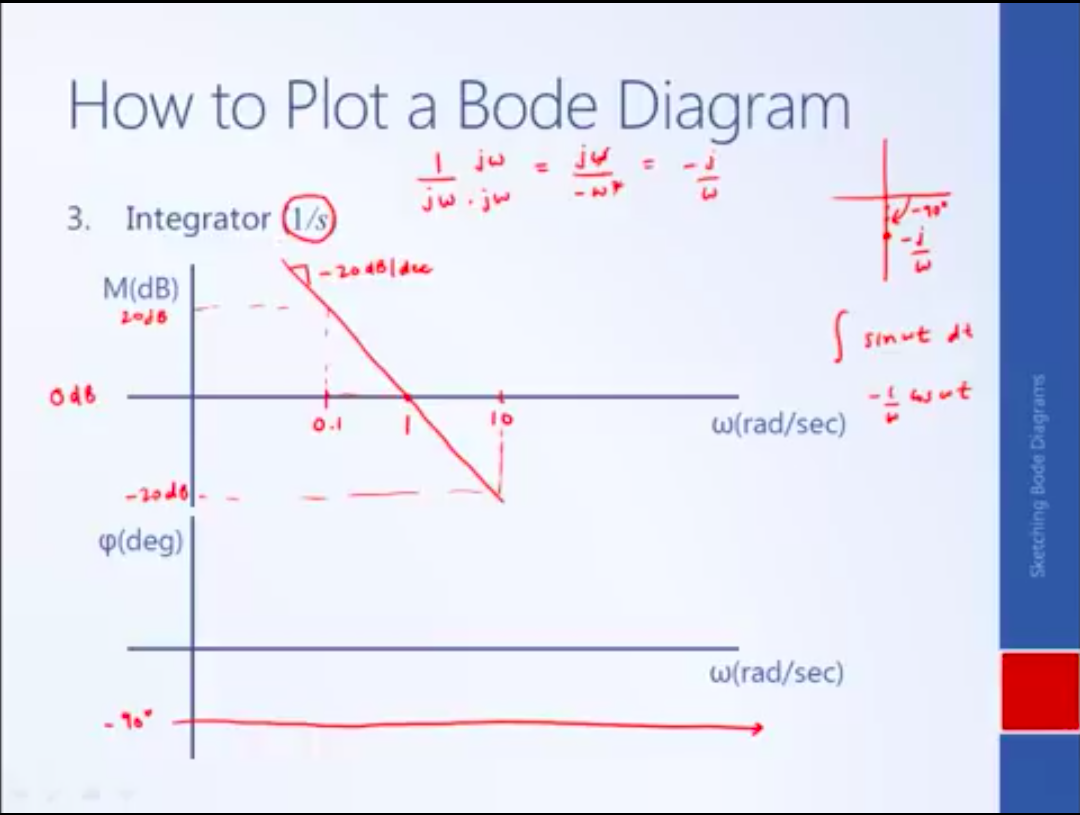
\includegraphics[width=\linewidth]{Bilder/FreqResp_BodePlot_1s}
	\caption{Bode plot of Integrator $1/s$}
	\label{Fig_FreqResp_BodePlot_1s}
\end{figure}
\newpage

Another intuition can be made in time-domain as $1/s$ is an integrator in time-domain, for an input frequency of sine wave, the input sine function as a function of $\omega$ $sin(\omega t)$ is integrated as follows:
\begin{equation}
\int sin(\omega t) = -\frac{1}{\omega} cos(\omega t)
\end{equation}
The negative cosine wave is always lagging by $90^{\circ}$ from the input sine wave. Also ,it can be seen that the magnitude is initially negative and increases towards the origin as per the ratio $-1 / \omega$. Another intuition from the above equation is that at low frequencies the magnitude of the system response if high, this results in high DC gain $K_{dc}$ of the system at low frequencies. Such high gain at low frequencies provides the sufficient system gain to over-come the steady-state error.

\subsubsection{Bode Plot for simple Zero}

For a case of simple zero the TF is written in the form $(Ts+1)$, this is called the Bode form. The magnitude and phase plots are determined by substituting $s = j \omega$. At low frequencies $Ts$ is very small and $1$ will be dominating, therefore the magnitude and phase response in Bode plot will be a flat line similar to a simple gain $K$ as shown in figure \ref{Fig_FreqResp_BodePlot_zero}.
\begin{figure}[h!]
	\centering
	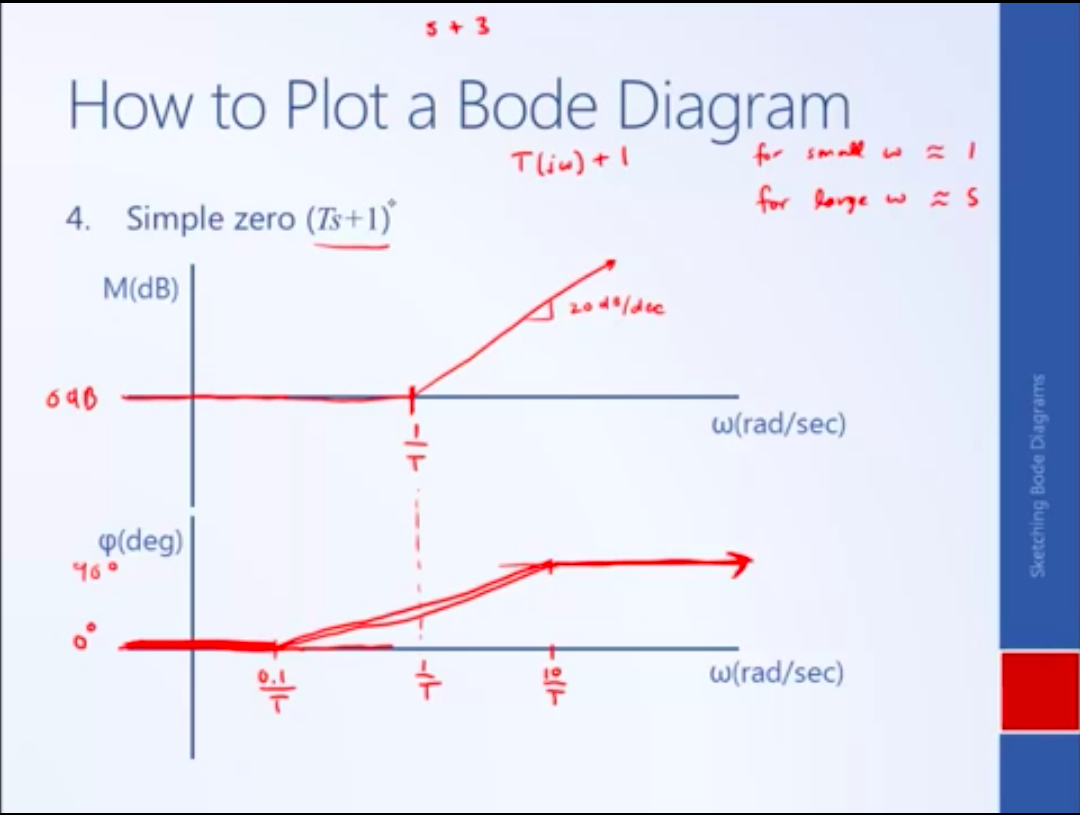
\includegraphics[width=\linewidth]{Bilder/FreqResp_BodePlot_zero}
	\caption{Bode plot of simple zero $(Ts + 1)$}
	\label{Fig_FreqResp_BodePlot_zero}
\end{figure}
At higher frequencies (higher vales of $\omega$), the term $Ts$ will be dominating and the multiplication of $s$ term in Laplace will result in differentiation in time-domain. Therefore, the magnitude and phase response in Bode plot will be similar to that of a differentiator $s$ as described previously. The magnitude will increase with a positive slope of $20 dB/decade$ and the phase will be leading with $90^{\circ}$ angle to the input as shown in figure \ref{Fig_FreqResp_BodePlot_zero}. In between these two lines the intermediate phase is a straight line approximation of a straight line connecting those two lines.

The cut-off point when the magnitude crosses over the $0 dB$ line is given by the ratio $1/T$ (I don't know why). For the phase plot, the slope starts at a decade earlier when $\omega = 1/T$ and ends a decade later after $\omega = 1/T$ as shown in figure \ref{Fig_FreqResp_BodePlot_zero}. 

\subsubsection{Bode Plot for simple Pole} \label{Sec_BodePlotSimplePole}

Similarly, in the case of a simple pole, the magnitude and phase response is determined by substituting $s = j \omega$. The TF of Bode form of a simple pole is expressed as:
\begin{equation}
	Simple Pole = \frac{1}{Ts + 1}
\end{equation}
substituting $s = j \omega$:
\begin{equation}
	\frac{1}{Ts + 1} = \frac{1}{T j \omega + 1}
\end{equation}
at lower input frequencies, the term $1$ will dominate the function and the output TF will just be $1$ and the magnitude in $dB$ will be $0$. The magnitude response is therefore, similar to a simple gain $K$. The phase similarly, behaves like a simple gain with phase $\phi = 0^{\circ}$ as in this case the simple gain is always positive. At higher frequencies the term $1/Ts$ will dominate and therefore, the output TF acts like an integrator in the time-domain. As it is with integrators, the magnitude will decrease with a negative slope of $- 20 dB/decade$ and the phase will have a constant lag of $-90^{\circ}$ with the input frequnvy $\omega$ as shown in figure \ref{Fig_FreqResp_BodePlot_pole}.
\begin{figure}[h!]
	\centering
	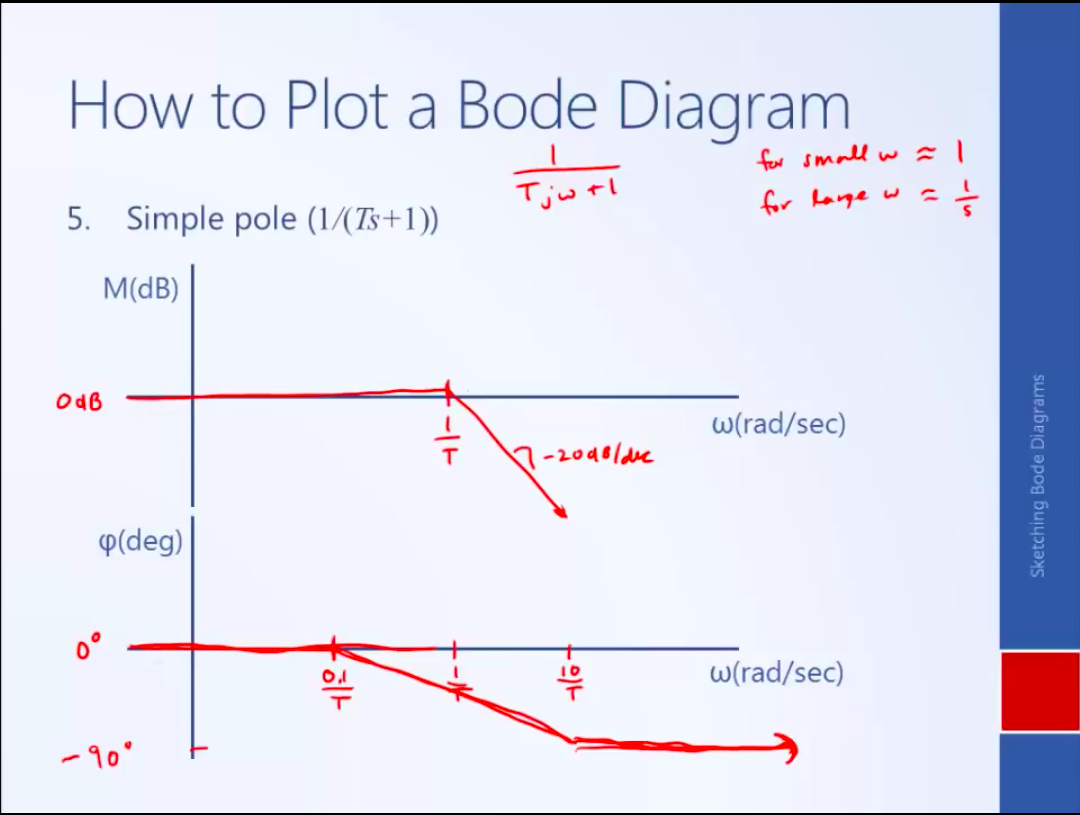
\includegraphics[width=\linewidth]{Bilder/FreqResp_BodePlot_pole}
	\caption{Bode plot of simple pole $1/(Ts + 1)$}
	\label{Fig_FreqResp_BodePlot_pole}
\end{figure}
The intermediate line between a contact gain term $1$ and a integrator term $1/Ts$ is approximated as a straight line. Similar to the differential plot, the break-off frequency $\omega$ at which the magnitude crosses-over the $0 dB$ line is at $1/T$ and the slope starts and ends a decade earlier $0.1/T$ and a decade later $10/T$ respectively as shown in figure \ref{Fig_FreqResp_BodePlot_pole}.

\textbf{Important notes: }As was seen in this section, that a simple pole acts like an integrator at higher frequencies, the effect of integrator eliminating ss-error seems like should be evident at higher frequencies. At lower frequencies therefore at additional integrator is added so that the effect of the integrator is already evident at lower frequencies eliminating ss-error.

\textbf{Important notes: }Unlike time-domain response (step input), in frequency response the effects of non-dominant poles (poles with faster settling times) can be clearly seen in the Bode plots. As the effects of such poles are evident at input $\omega$ of higher frequencies. In time-domain analysis, the input frequency is very low and the effects of poles with faster settling times is not captured. As at higher frequencies the speed (frequencies) of the input waves become faster the effect of the faster poles start to show up as a result of high speeds (frequencies).

Approach for drwaing Bode plots:
\begin{enumerate}
	\item Put the components (gain, diff, int, zeros and poles) in the Bode form
	\item Sketch the straight line approximations of the components on the Bode plot
	\item Add the graphs
	\item Try to approximate the curves
\end{enumerate}
Step 4 is optional as an accurate Bode plot is always possible with Matlab.

\section{Stability analysis from Frequency response}

From time-domain analysis, it was found that based on the position of poles from the imaginary axis, the systems stability could be defined weather it is stable or unstable or marginally stable (such as in the case of defining BIBO stability. Further assigning degree of stability such as asymptotic stability (where the system is perfectly stable and all oscillations will damp out to zero), another degree of stability term is used in the frequency domain analysis called \textbf{\textit{relative stability}}.

Relative stability is the degree of stability of the system determined knowing the positions of the poles from the imaginary axis. As the systems with poles located far away from the imaginary axis is much more stable, damping out the oscillations quickly and have faster settling times than the systems that have their poles located closer to the imaginary axis.

Additionally, to the system stability definitions derived in the time-domain analysis using the pole positions, stability of the system can be defined using frequency based analysis as well. It turns out that the stability is defined in much better way using frequency response of the system.

\subsection{Relative Stability: How far is the system from going unstable}

The stability of closed-loop system can also be determined from the open-loop frequency response. Consider a closed-loop system as shown in figure \ref{Fig_FreqResp_RelStabil_1}.
\begin{figure}[h!]
	\centering
	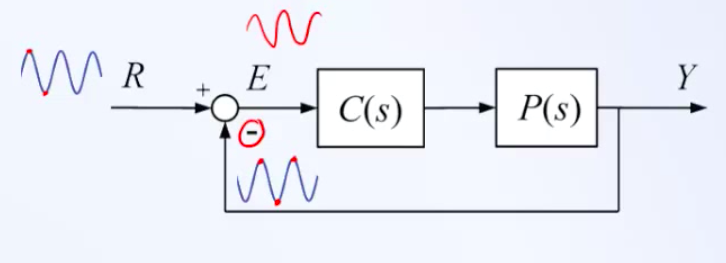
\includegraphics[width=0.8\linewidth]{Bilder/FrequencyResp_ClosedLoopSystem}
	\caption{A Closed-loop system with input as frequency}
	\label{Fig_FreqResp_RelStabil_1}
\end{figure}
\newpage
The input to the system is in form of frequency, therefore, the system would react from the error signal that is also of the shape of the input signal.

\textbf{Note: }When summing two frequencies, the resulting frequency is of the same shape as the first frequency.

If the open-loop response of the system has a frequency that is completely out of phase $(\phi = 180^{\circ})$, this will lead to addition of the two signals and therefore, the magnitude of the error is more than 1 (1 is the magnitude of the reference signal). If the open-loop attenuates the signal, then this is not a problem as the magnitude of error though greater than 1 will start to subside. However, if the open-loop amplifies the signal, then the feedback would add and amplify the error signal again and again (error signal grows exponentially) causing the actuator to saturate at its peak and the system as a whole going unstable. 

The above theory can be visualized mathematically taking two sinusoids $A e^{-\sigma t} sin(\omega t)$ and $B e^{-\sigma t} sin(\omega t + \phi)$. Where $A e^{-\sigma t}$ is the amplitude (envelope) of the sine wave $sin(\omega t)$ given as a variable of time $t$. In case of . Because of the summation (let the amplitude $A =B = 1$), the two signals become:
\begin{align}
	\sum e(t) 	&= e^{-\sigma t} sin(\omega t) - e^{-\sigma t} sin(\omega t - \phi) \\
				&= 2 e^{-\sigma t} sin(\omega t) \label{Eq_ConstructiveInterference}
\end{align}

\textbf{Note: }The above equation was constructed by me and is not an accurate mathematical description of error signal at the summation point. The above result is generated using $\phi = \pi$, the $180^{\circ}$ phase lag.

As can be seen from equation \eqref{Eq_ConstructiveInterference}, the error signal becomes double the reference signal instead of going to zero (this would be the case when the signal was in phase, then the summation becomes negative in equation \eqref{Eq_ConstructiveInterference}). This error signal $r(t) = 2 e^{-\sigma t} sin(\omega t)$ if amplified in the system (due to gain $K + $), then it will be added and amplfied again and again in the loop (exponential increase). Such a phenomena is also called \textbf{\textit{constructive interference}}.

When the OL response of the system is out-of-phase from the reference signal, then the error would actually add up as given by the previous equation instead of having the difference between them. The signal can then be amplified or attenuated by the controller based on the gain $K$. So how far can the control gain be given before the system goes unstable due to error signal going from attenuation to amplification?

\subsubsection{Defining Relative stability}

With the theory laid down in the previous section, relative stability can be defined based on how far the open-loop frequency response of the system is to phase lag of $180^{\circ}$ and a magnitude of $1$.

Specifically, terms can be defined that are useful for defining relative stability:
\textbf{Gain Margin $G_m$}: Says when the OL response is at a phase lag of $180^{\circ}$, how much gain can be given to the system before it starts to amplify?
Specifically, $G_m$ is the distance from the magnitude of $1 (0 dB)$ at the frequency where $\phi = -180^{\circ}$ (phase cross-over frequency).

\textbf{Phase Margin $\phi_m$}: Says, when we are at the OL-response magnitude of $1 or (0 dB)$, then how far is the OL-response phase from the $-180^{\circ}$ out-of-phase frequency.
Specifically, $\phi_m$ is the distance from the phase of $-180^{\circ}$ at the frequency where $M = 0 dB$ (gain cross-over frequency). Both the gain and the phase margins can be understood from the graphical figure shown in \ref{Fig_FrequencyResponse_GainAndPhaseMargins}.
\begin{figure}[h!]
	\centering
	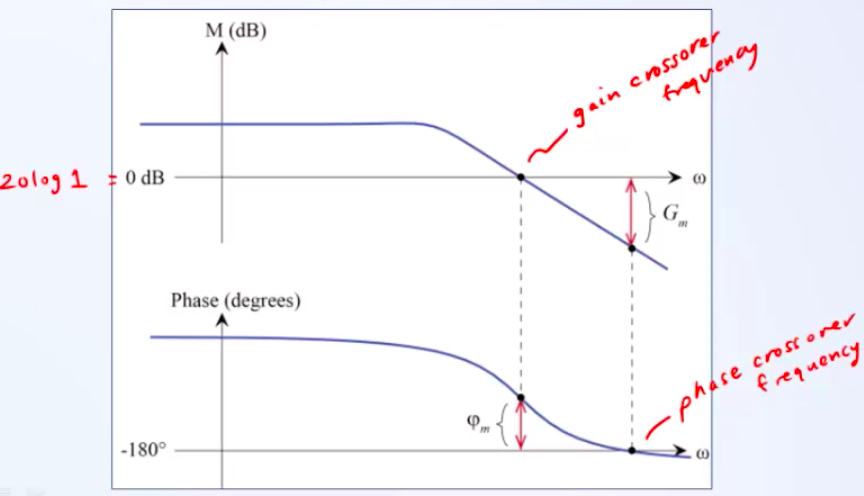
\includegraphics[width=\linewidth]{Bilder/FrequencyResp_GainAndPahseMArgins}
	\caption{Gain and phase margins on Bode plot}
	\label{Fig_FrequencyResponse_GainAndPhaseMargins}
\end{figure}

Also, it should be noted from figure \ref{Fig_FrequencyResponse_GainAndPhaseMargins}, that both the gain and phase margins should be positive in order for the system to be stable. As can be seen in figure \ref{Fig_FrequencyResponse_GainAndPhaseMargins}, at phase cross-over frequency, the magnitude is under $0 dB$, if gain is made negative the magnitude will cross over or at least reach $0 dB$ therefore, crossing over from attenuation to amplification that might cause resonance and actuator saturation (undesired behavior). Also, in case of phase, the phase is already in the negative region same as the magnitude any more negative phase will tend the frequency (OL) towards $-180^{\circ}$ (out-of phase).

As can be seen from figure \ref{Fig_FrequencyResponse_GainAndPhaseMargins}, when the OL system response is out-of-phase, then the OL magnitude is attenuated and is less than $0 dB$. Therefore, the errors signal should also be less than the reference signal. This is the case for the given system gain $K$. If the control gain $K$ is changed such a way that the OL magnitude becomes $0 dB$ then the error signal will now becomes double of the reference signal as given by equation \eqref{Eq_ConstructiveInterference}. From here, the systems response would be added and multiplied by the feedback, causing the system to go unstable. Now, the margin of control gain $K$ that we can alter such that OL system magnitude reaches $0 dB$ is called the \textbf{\textit{gain margin}}. The similar analogy is true for \textbf{\textit{phase margin}}.

In order to visualize the effect of $K$ in eating up the gain margin $G_m$, consider the figure \ref{Fig_FrequencyResp_K4Gm}.
\begin{figure}[h!]
	\centering
	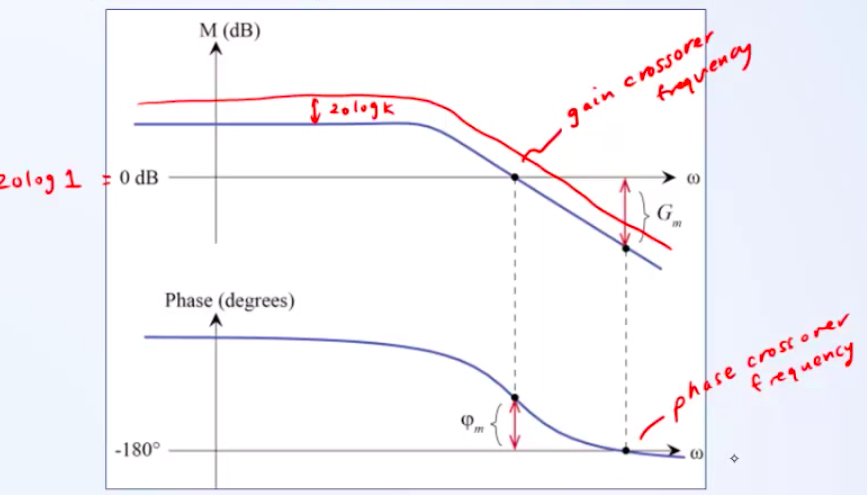
\includegraphics[width=\linewidth]{Bilder/FrequencyResp_K4Gm}
	\caption{Effect of $K$ on relative stability}
	\label{Fig_FrequencyResp_K4Gm}
\end{figure}
In Bode plots when two components are connected in series their system response is added up in the Bode plot. Here, the plant $G(s)$ is in series with the controller $C(s)$ which has a gain $K$. Depending on the numerical value of $K$, the response due to $K$ on Bode plot is a straight line given by $20 log_{10}K$ (adding $20 log_{10}K$ with the blue line) which would amplify or attenuate the OL response magnitude. In case changing $K$ attenuates the OL response magnitude, such a scenario is shown in figure \ref{Fig_FrequencyResp_K4Gm}. Therefore, in this case $K$ eats up $G_m$, the limit beyond which the system is unstable.

\section{Caclulation of gain and phase shifts}

For a given systems response, the gain amplification / attenuation along with the phase shift is determined at its \textbf{\textit{steady-state response}}. As an example, the following calculation is performed in order to determine the response parameters (magnitude and phase shift) as shown in figure \ref{Fig_FrequencyResp_ExampleProb}.
\begin{figure}[h!]
	\centering
	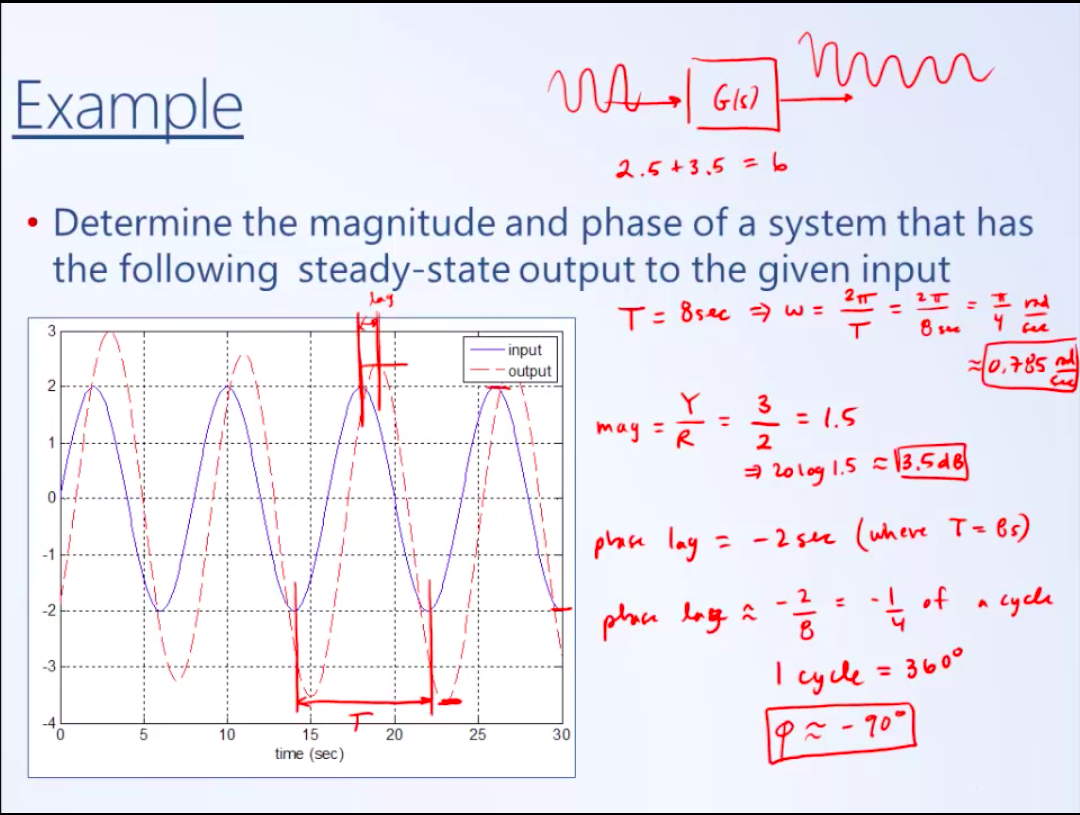
\includegraphics[width=\linewidth]{Bilder/FrequencyResp_ExampleProb}
	\caption{Determining Magnitude and Phase using Bode Plots}
	\label{Fig_FrequencyResp_ExampleProb}
\end{figure}

Once the response (attenuation/amplification and phase) is determined for one such input frequency, the process is repeated at every input frequency and all the data points are plotted on the \textbf{\textit{Bode Plot}}. 

\subsection{System Indentification using Bode Plots}

In another example shown in figure \ref{Fig_FrequencyResp_ExampleProb2}, the TF of the system is determined using only the Bode plots (open-loop Bode Plot) of the system. This example is performed in order to establish various parameters that can be identified using only the Bode plots or Frequency response of the system. The following method is generally employed in \textbf{\textit{System Identification}} methods. In Matlab however, there is this in-built program which does all this automatically, however, it is very important to understand the analytical basis of system identification method described for identifying control systems.
\begin{figure}[h!]
	\centering
	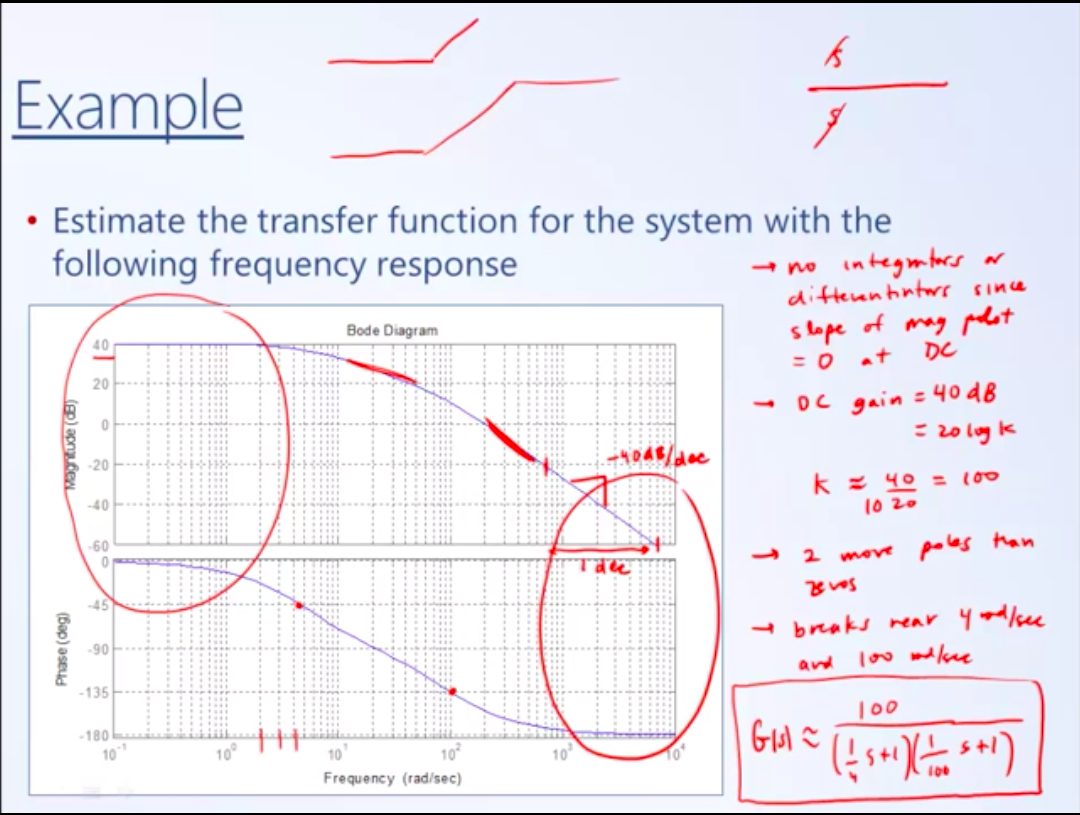
\includegraphics[width=\linewidth]{Bilder/FreqResp_Example2}
	\caption{system Identification using Bode Plot}
	\label{Fig_FrequencyResp_ExampleProb2}
\end{figure}

The first step in to determine the presence of integrators and differentiators in the system by examining the low frequency response. Since an integrator or the differentiator will always produced a negative or a positive slope respectively right from the beginning, it is easier to notice their presence. In our case as shown in figure \ref{Fig_FrequencyResp_ExampleProb2}, this is not the case as the line is flat at low frequencies and the slope at medium to high frequencies is due to the poles. Therefore, this system has no integrators or differentiators or in other words, there are no poles or zeros at the origin.

The second step is to determine the DC gain $K_{dc}$ of the system. The DC gain is the ss-response of the system at low frequencies with a constant input (step input). From the low frequency response of the system, it can be seen that the DC gain is $40 dB$. From this the DC gain can be expressed in the non-logarithmic scale by taking anti-log (anti-log of base 10 is 10 raise to power) as 

$$	40 dB = 20 log K \implies K = 10^{40/20}=100	$$

The third step in to detemrine the number of poles and zeros. The relative number of poles in the system that are more than zeros can be determined using the high frequency response in the Bode plots. That is, the number of poles that are more than zeros. From the high frequency response shown in figure \ref{Fig_FrequencyResp_ExampleProb2}, it can be seen that there are two poles in the system more than zeros which can be verified using both the magnitude and phase response. From Magnitude response the ss-response has a slope of $- 40 dB/decade$, which is the case for two poles as each poles produce a slope of $-20 dB /decade$. Additionally, from the phase plot it can be seen that the phase shift at higher frequencies has shifted to about $-180^{\circ}$. As is the case with each pole the phase shifts to about $-90^{\circ}$. Sometimes, it is also said that there are zeros also in the numerator but they have been canceled out by the poles in the denominator. The cancelled out poles and zeros could be either at origins (integrators and differentiators) or simple poles and zeros (non origin). Either way, as the zeros cancel out, using Model Reduction technique it could be said that since their effect is not present, there is no need to include their dynamics and cancel them again later.

The fourth step is to determine the location of the poles. It is rather difficult to determine this manually using Bode plots, however, a rough estimation can be provided. Using Matlab the precise locations of the poles can be determined. From the magnitude plot the breaks points of the poles where the response starts to slope (as described in section \ref{Sec_BodePlotSimplePole}) due to the presense of poles. it can be seen that the break point $(1/T)$ can rougly be noticed at $4$ rad/s where magnitude slope is roughly $-20 dB /decade$ and the mid point $45^{\circ}$ of the phase plot occurs at $4$ rad/s. Similarly, the midpoint of phase plot for the second pole where the phase goes from $-90^{\circ}$ to $-180^{\circ}$ is clearly at $100$ rad/s. Also noting that the magnitude plot slopes roughtly to $-40 dB/decade$ from this point. Writing the poles in the bode form and using the DC gain deterimed previosly, the following TF can be expressed for the given Frequency response:
\begin{equation}
	G(s) = \frac{K_{dc}}{(s + z_1)(s + z_2)} = \frac{100}{(\frac{1}{4}s + 1)(\frac{1}{100}s +1)}
\end{equation}

\section{Nyquist Diagram}

A Nyquist diagram visualizes the information of the frequency response of the open-loop system on a single plot unlike in Bode plots where different plots are used. A Nyquist plot is useful for feedback loop analysis and design. Unlike in Bode plots, the gain and phase margins of a complex number $G(j\omega)$ is not considered separately in Nyquist plots. Instead, the complex number is taken as given and a plot of $G(j\omega)$ is generated on the complex plane, for all real values of $\omega$. However, in the long run, a plot of $-\omega$ is also generated to complete the sketch.

For calculating the a simple complex number for a vector of $\omega$, the following approach is used:
\textbf{Inverting a complex number}
\begin{equation*}
	G(j\omega) = \frac{1}{j \omega + 1} = \frac{1}{j \omega + 1} \frac{j \omega - 1}{j \omega - 1} = \frac{j \omega - 1}{-\omega^2 - 1} = \frac{1 - j\omega}{1 + \omega^2}
\end{equation*}

However, when the calculation for simplifying the complex number is complex, then magnitude and phase equations derived in Bode plots can be used as given by equations \eqref{Eq_FeResMagEquation} and \eqref{Eq_FeResMagEquation} respectively. Then the complex number can be determined by combining magnitude and phase values calculated from equations \eqref{Eq_FeResMagEquation} and \eqref{Eq_FeResMagEquation}. For $m$ the magnitude and $\phi$ the phase of the complex number, the complex number itself can be calculated using either the \textbf{\textit{phasor form}} or the \textbf{\textit{component form}}.
\textbf{\textit{phasor form}}:
\begin{equation}
	complex num = m e^{j \phi}	
\end{equation}
\textbf{\textit{component form}}:
\begin{equation}
	complex num = m cos\phi + j m sin\phi
\end{equation}
In case of using computing softwares not capable of handling complex numbers, component form is more suitable and in case of analytical calculations, phasor form is more suitable as it is easier with multiplication and division.

\subsection{An example of plotting Nyquist plot for a simple system}

Consider a open-loop of a simple system given by:
\begin{equation}
	G(s) = \frac{1}{s + 1}
\end{equation}
The complex numbers can be calculated for each of the input $\omega$ using either of the two methods described above and a table can be constructed containing vectors of input $\omega$ and the calculated complex number as shown below:
\begin{table}[h!]
	\centering
	\begin{tabular}{m{4cm} | m{4cm}}
		\toprule
		$\omega$ & $G(j\omega)$ \\
		\cmidrule{1-2}
		0.1 & 0.99 - 0.99j \\
		0.5 & 0.8 - 0.4j \\
		1 & 0.5 - 0.5j \\
		2 & 0.2 - 0.4j \\
		10 & 0.01 - 0.1j\\
		\bottomrule
	\end{tabular}
	\caption{Table showing $G(j\omega)$ calculation for Nyquist plot}
	\label{Tab_Gjw_calculation_NyquistPlot}
\end{table}
A Nyquist plot generated for the complex numbers given in table \ref{Tab_Gjw_calculation_NyquistPlot}, is plotted using Matlab as shown in figure \ref{Fig_FrRes_NyquistEx1}
\begin{figure}[h!]
	\centering
	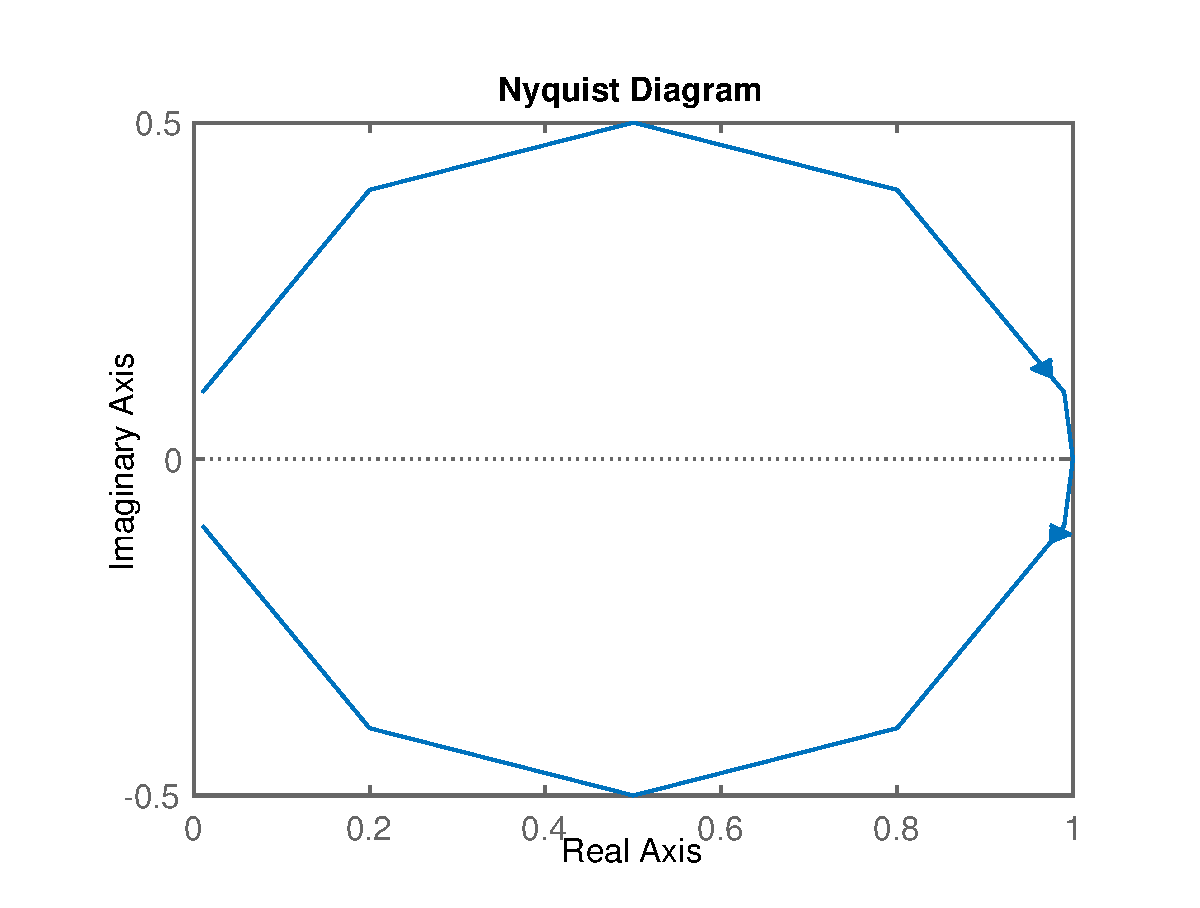
\includegraphics[width=0.7\linewidth]{Bilder/FrRes_NyquistEx1.eps}
	\caption{Plotting example of complex numbers in Nyquist plot}
	\label{Fig_FrRes_NyquistEx1}
\end{figure}
\newpage
Figure \ref{Fig_FrRes_NyquistEx1} also contains $-\omega$ shown in the upper half plane.